\section{Vorbereitung}

\noindent{\large Arbeitsaufteilung:\par}
\begin{table}[htb]
\centering
\caption{Arbeitsaufteilung in der Gruppe}
\label{Arbeitsaufteilung}
\begin{tabular}{c|ccc}
\toprule
Aufgabe & Lucas & Aleksandra & Timo\\
\midrule
Motivation &  & x & \\
Literaturrecherche & x &  & \\
1.2 Vermessung & x & x & x\\
1.3 Langzeitmessung & x & x & x\\
1.4 Energiespeicherung & x & x & x\\
1.5 Vergleich &  &  & x\\
Dokumentation & x & x & x\\
Diskussionen & x & x & x\\
Bericht \& Matlab & x &  & \\
\bottomrule
\end{tabular}
\end{table}

\noindent{\large Genutzte Materialien:\par}
\begin{table}[htb]
\centering
\caption{Genutzte Materialien}
\label{Arbeitsaufteilung}
\begin{tabular}{c|c|c}
\toprule
Bauteiltyp & Beschreibung & Wert\\
\midrule
Solarzelle & SEEED Studio POW112D2P & $U_{OC} = \SI{5,5}{\volt}, I_{SC} = \SI{4}{\milli\ampere}$ bei $\SI{5}{\kilo\lux}$\\
Zener-Diode & ZF 5,1; 5,1V 0,5W & V = 5,1V; P = 0,5W\\
Speicherkondensator & Panasonic 5,5V 220mF & V = 5,5V; C = 220,0mF\\
Stützkondensator & Keramikkondensator Code 104 & C = 100,0 nF\\
Widerstand & Kohleschichtwiderstände & $\SI{10}{\ohm} - \SI{10}{\mega\ohm}; P = 025W; 5\%$\\
Steckbrett & Breadboard & \\
Drahtbrücke & Drahtbrücken-Set 140-teilig & \\
\bottomrule
\end{tabular}
\end{table}

\clearpage
\section{Einleitung}

\subsection{Motivation}
Ein sehr wichtiger Aspekt jeder Lehre ist die sowohl theoretische als auch praktische Beschäftigung mit dem zu lernenden Stoff. Diesen Zweck erfüllten die Aufgaben dieses Workshops.
\\
\\
Wir hatten die Gelegenheit dazu uns mit einer erneuerbaren Energiequelle in Form einer Solarzelle in der Praxis auseinanderzusetzten und Messungen druchzuführen. Dabei haben wir im Zuge der Rechnerche gelernt, welche Arten von Energiequellen es gibt und deren Vor- und Nachteile ermittelt. 
\\
\\
Im Zuge des Workshops wurden von uns verschiedene Messungen durchgeführt, Aufgaben gelöst und Diskussionen durchgeführt, was unsere Zusammenarbeit forderte und unser Wissen bezüglich erneuerbarer Energiequellen erweiterte. Mithilfe eines Microcontrollers und der vorgegeben Schaltungen führten wir Messungen durch, analysierten anschließend unsere Messergebnisse und formulierten daraus folgende Resultate. Das Lösen der Aufgaben hat des Weiteren unser logisches Denken gefordert.
\\
\\
Unsere Kenntnisse gingen über die Elektrotechnik hinaus, denn wir haben unsere Kentnisse in Matlab, LateX und lenlab vertieft. Diese grundlegende Vertiefung kam durch das selbststädnige Erlernen und Ausprobieren zustande.

\subsection{Literaturrecherche}
Erneuerbare Energien spielen schon heute und besonders für die Zukunft unserer modernen Gesellschaften eine große und tragende Rolle. Dabei unterscheiden sie sich im Vergleich zu den endlichen Ressourcen unseres Planeten wie zum Beispiel Erdöl oder Kohle, da sie ''im Rahmen des menschlichen Zeithorizonts praktisch unerschöpflich zur Verfügung stehen oder sich verhältnismäßig schnell erneuern''. \cite{wikipedia_erneuerbare}

Die Vertreter der regenerativen Energieerzeugung sind dabei die Windkraft (z.B.: Windkraftanlage), die Wasserkraft (z.B.: Staudamm), die Geothermie (z.B.: geothermisches Kraftwerk), die Bioenergie (z.B.: Biogas) und wie in diesem Workshop näher betrachtet die Solarenergie mit dem Schwerpunkt Photovoltaik als Beispiel.

Betrachtet man die Vorteile der regenerativen Energien, so fallen einem direkt zwei auf: \cite{focus_procontra}
\begin{itemize}
\item Die regenerativen Energien liegen bei optimalen Bedingungen (z.B.: Sonnenlicht, Wind) quasi unbegrenzt vor oder regenerieren sich sehr schnell. Global gesehen wird die Erde ständig von der Sonne beleuchtet, somit kann Sonnenergie rund um die Uhr in Energie umgewandelt werden.
\item Die Möglichkeiten der erneuerbaren Energien sind sehr vielfältig und können so regional und ohne großen Transport genutzt werden.
\end{itemize}

Im Vergleich dazu sind die Nachteile minimal: \cite{focus_procontra}
\begin{itemize}
\item Die Anschaffungen zur Gewinnung der erneuerbaren sind zum jetzigen Zeitpunkt noch teuer. Mit neuen Technologien werden die Preise aber fallen.
\item Die Leistung und Energie, welche durch erneuerbare Energien gewonnen werden kann, ist oft weitaus geringer als die gewonnene Leistung der endlichen Energiequellen (Beispiel Atomkraftwerk)
\end{itemize}

Wie funktioniert die Gewinnung elektrischer Energie mit Hilfe von Photovoltaik?
\begin{itemize}
\item Bei der Energiegewinnung durch Photovoltaik werden von der Siliziumsolarzelle Photonen ("Lichtteilchen") aufgenommen und in elektronische Ladungsträger umgewandelt. Diese werden nun nach ihrer positiven und negativen Ladung getrennt und zu den zwei äußeren Elektroden transportiert. Dabei entsteht zwischen diesen eine elektrische Spannung. \cite{weltderphysik}
\end{itemize}

Was beschreibt die I-U-Kennlinie und was versteht man unter dem Maximum-Power-Point (MPP) einer Solarzelle?
\begin{itemize}
\item Die I-U-Kennlinie beschreibt die Stromstärke pro Spannung der Solarzelle, d.h. den Innenwiderstand der Zelle.
\item Der MPP einer Solarzelle beschreibt den Punkt, an welchem die Solarzelle die maximale Leistung abgibt. Dieser Punkt kann auf der I-U-Kennlinie gefunden werden, wenn das Rechteck mit der Höhe = I und der Breite = U maximal ist. \cite{Fachkundebuch}
\end{itemize}

Welche Möglichkeiten zur Speicherung von (regenerativ erzeugter) elektrischer Energie gibt es?
\begin{itemize}
\item Die Möglichkeiten der Energiespeicherung sind sehr vielfältig. Dazu gehören thermische (z.B.: Wärmespeicher), chemische (z.B.: Wasserstoff), mechanische (z.B.: Feder, Pumpspeicherkraftwerk) und elektrische (z.B.: Kondensator) Speicher.
\end{itemize}

\clearpage
\section{Aufgaben}

%Aufgabe 2
\subsection{Vermessung der Solarzelle POW112D2P}

Für die ganze Aufgabe 2 wurde die folgende Schaltung verwendet:

\begin{figure}[htb]
\centering
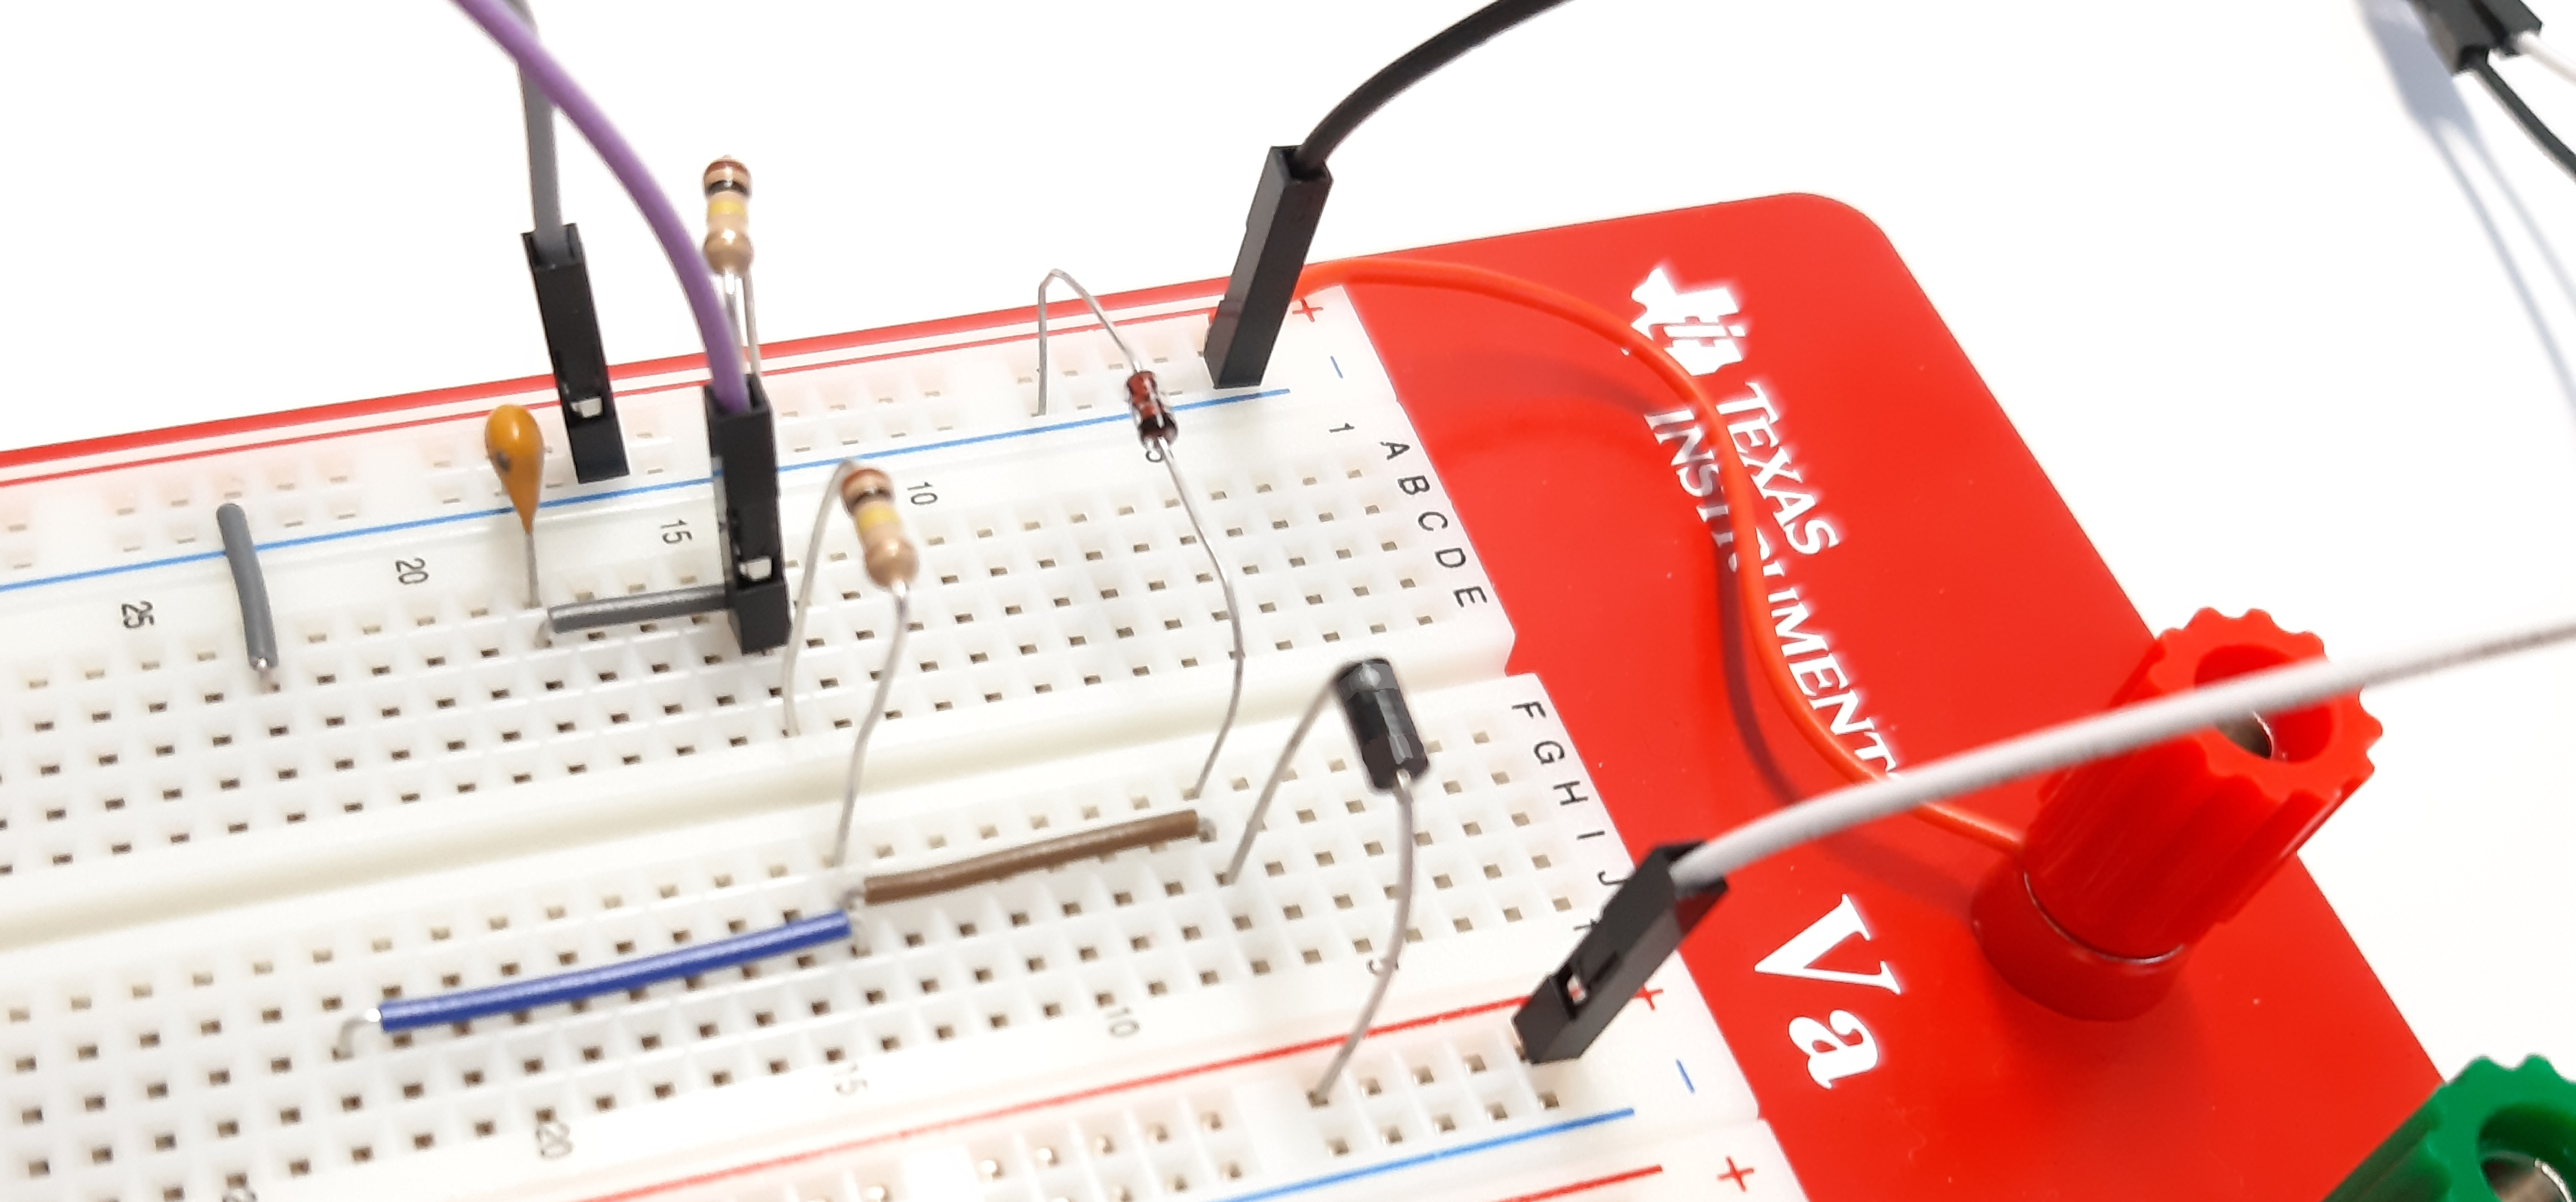
\includegraphics[width=16cm]{pictures/Dokumentation/Schaltung-1.jpg}
\caption{Aufbau der Schaltung für die Aufgabe 2}
\label{fig:Schaltung2}
\end{figure}

Bekannte Verhältnisse:
\[
I_{ges} = \frac{U_{ges}}{R_{ges}}
\]
\[
U_{ges} = 2 * U_{mess}
\]
\[
R_{mess} = R_{1} + R_{2}
\]
\[R_{ges} = \frac{R_{mess} * R_{L}}{R_{mess} + R_{L}}\]

\[
\Rightarrow I_{ges} = \frac{U_{ges}}{R_{ges}} = \frac{2 * U_{mess}}{\frac{R_{mess} * R_{L}}{R_{mess} + R_{L}}} = \frac{(2 * U_{mess}) * (R_{mess} + R_{L})}{R_{mess} * R_{L}}
\]

\[P = U * I = U * \frac{U}{R} = \frac{U^2}{R}\]

\clearpage
\subsubsection{Aufnehmen der I-U-Kennlinie}

\noindent{\Large Materialien:\par}

In dieser Teilaufgabe messen wir die abgegebene Spannung der Solarzelle in Abhängigkeit von wechselnden Lastwiderständen.
Wir erwarten höhere Spannungswerte bei steigenden Lastwiederstandswerten (außer bei $R_{L} = 0$).
Ab einem gewissen Lastwiederstand erwarten wir einen drastischen Aufstieg der Messwerte, welche dann gegen die Leerlaufspannung ($R_{L} = 0$) tendieren.
Aus der gemessenen Spannung und dem bekannten Gesamtwiderstand berechnen wir die Stromstärke mit der oben genannten Formel.
\\
\\
Wir vernachlässigen dabei den Spannungsabfall über der Diode und über den Leitungen.
\\
\\
Das folgende Matlab-Skript wurde zur Berechnung von $I_{ges}$ und der Ausgabe der Kennlinien geschrieben:
\lstinputlisting[caption = Funktion \textit{UIKennlinien.m}., label = UIKennlinien.m]{matlab/UIKennlinien.m}

\clearpage
\noindent{\Large Durchführung:\par}

\begin{table}[htb]
\centering
\caption{Messungen mit einer Leuchtstoffröhre (ca. 18W) mit 2m Abstand und einem Winkel von $\ang{90}$}
\label{Leuchtstoffröhre}
\begin{tabular}{cc}
\toprule
Widerstand [$\Omega$] & Gemessene Spannung [V]\\
\midrule
$0$ & $1.53$\\
$100$ & $0.0155$\\
$150$ & $0.0255$\\
$220$ & $0.04$\\
$470$ & $0.09$\\
$570$ & $0.11$\\
$680$ & $0.125$\\
$780$ & $0.145$\\
$830$ & $0.155$\\
$1000$ & $0.18$\\
$1150$ & $0.21$\\
$1220$ & $0.23$\\
$1500$ & $0.275$\\
$2200$ & $0.38$\\
$3300$ & $0.58$\\
$4300$ & $0.7$\\
$5020$ & $0.77$\\
$8200$ & $1.2$\\
$10000$ & $1.3$\\
$15000$ & $1.45$\\
$20000$ & $1.5$\\
$40000$ & $1.52$\\
\bottomrule
\end{tabular}
\end{table}

\begin{figure}[htb]
\centering
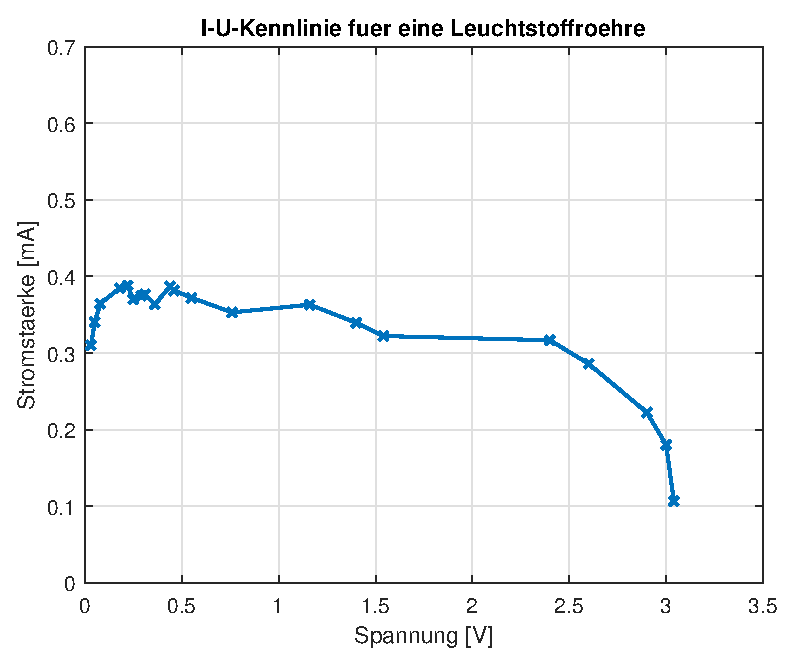
\includegraphics[width=8.5cm]{pictures/I-U/Leuchtstoffroehre-UI.eps}
\caption{I-U-Kennlinie einer Leuchtstoffröhre}
\label{fig:I_U_Leuchtstoffroehre}
\end{figure}

\clearpage
\begin{table}[htb]
\centering
\caption{Messungen mit einer Taschenlampe (ca. 10W) mit 10cm Abstand und einem Winkel von $\ang{90}$}
\label{Taschenlampe}
\begin{tabular}{cc}
\toprule
Widerstand [$\Omega$] & Gemessene Spannung [V]\\
\midrule
$0$ & $2.1$\\
$100$ & $0.034$\\
$150$ & $0.052$\\
$220$ & $0.075$\\
$470$ & $0.16$\\
$570$ & $0.19$\\
$680$ & $0.23$\\
$780$ & $0.255$\\
$830$ & $0.27$\\
$1000$ & $0.32$\\
$1150$ & $0.354$\\
$1220$ & $0.38$\\
$1500$ & $0.48$\\
$2200$ & $0.64$\\
$3300$ & $0.9$\\
$4300$ & $1.08$\\
$5020$ & $1.2$\\
$8200$ & $1.45$\\
$10000$ & $1.55$\\
$15000$ & $1.75$\\
$20000$ & $1.9$\\
$40000$ & $2$\\
\bottomrule
\end{tabular}
\end{table}

\begin{figure}[htb]
\centering
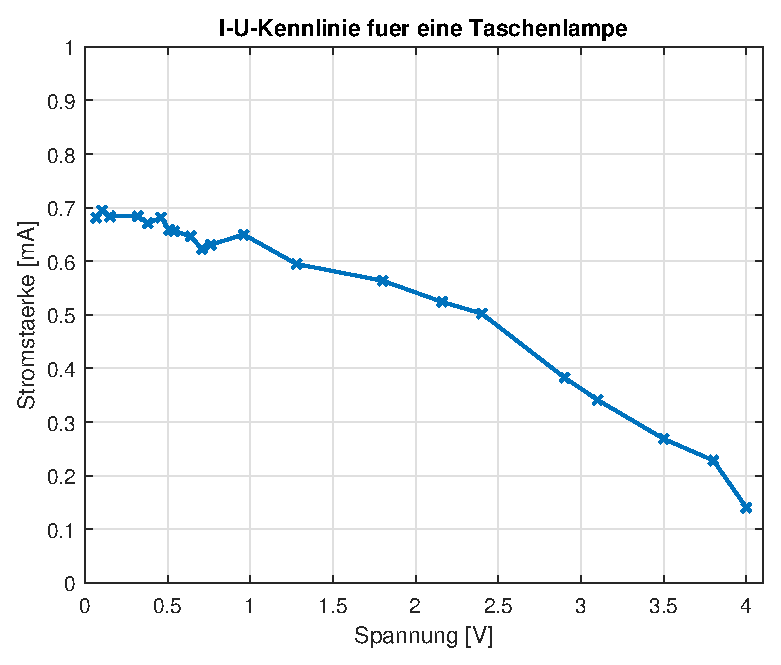
\includegraphics[width=9.5cm]{pictures/I-U/Taschenlampe-UI.eps}
\caption{I-U-Kennlinie einer Taschenlampe}
\label{fig:I_U_Taschenlampe}
\end{figure}

\clearpage
\begin{table}[htb]
\centering
\caption{Messungen mit einer Schreibtischlampe (ca. 20W) mit 20cm Abstand und einem Winkel von $\ang{90}$}
\label{Schreibtischlampe}
\begin{tabular}{cc}
\toprule
Widerstand [$\Omega$] & Gemessene Spannung [V]\\
\midrule
$0$ & $1.75$\\
$100$ & $0.0165$\\
$150$ & $0.025$\\
$220$ & $0.0365$\\
$470$ & $0.075$\\
$570$ & $0.0885$\\
$680$ & $0.11$\\
$780$ & $0.125$\\
$830$ & $0.13$\\
$1000$ & $0.155$\\
$1150$ & $0.18$\\
$1220$ & $0.19$\\
$1500$ & $0.24$\\
$2200$ & $0.35$\\
$3300$ & $0.51$\\
$4300$ & $0.65$\\
$5020$ & $0.75$\\
$8200$ & $1.15$\\
$10000$ & $1.225$\\
$15000$ & $1.425$\\
$20000$ & $1.55$\\
$40000$ & $1.6$\\
\bottomrule
\end{tabular}
\end{table}

\begin{figure}[htb]
\centering
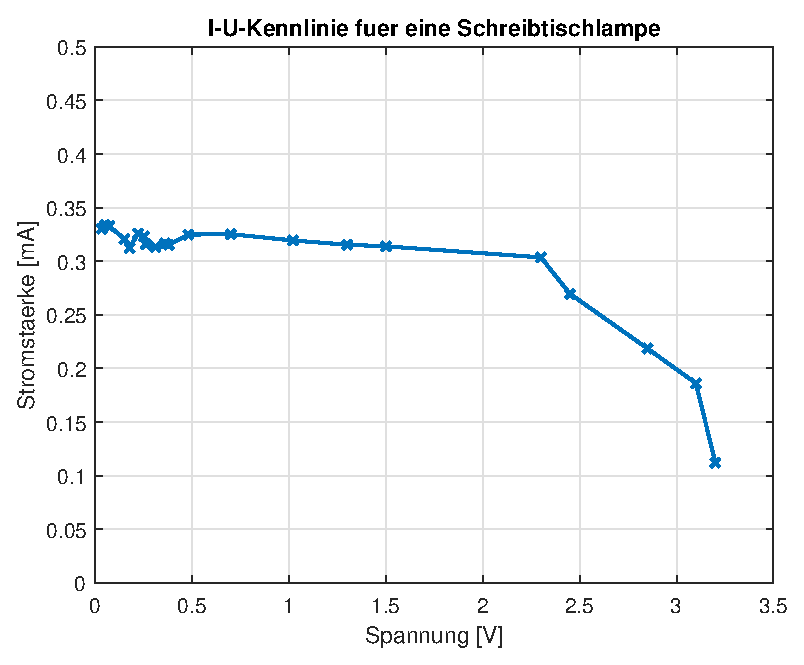
\includegraphics[width=9.5cm]{pictures/I-U/Schreibtischlampe-UI.eps}
\caption{I-U-Kennlinie einer Schreibtischlampe}
\label{fig:I_U_Schreibtischlampe}
\end{figure}

\noindent{\Large Diskussion:\par}

Abgesehen von wenigen Messungenauigkeiten entsprechen unsere Messwerte unseren Erwartungen.
Die Messfehler lassen sich auf Bauteiltoleranzen oder minimal wechselnde Lichtverhältnisse zurückführen.
Außerdem weist jede I-U-Kennlinie einen merklichen Knick auf, zu dessen Beginn wir den jeweiligen MPP vermuten.

\subsubsection{Bestimmung des Maximum-Power-Points (MPP)}

\noindent{\Large Materialien:\par}

Wir errechnen in Matlab die abgegebene Leistung der Solarzelle in Abhängigkeit der Widerstände mit der oben genannten Formel.
Wir erwarten die jeweiligen MPP dort, wo die I-U-Kennlinie anfängt zu knicken, da dort Spannung und Strom maximal sind.

Matlab-Skripte zur Berechnung der Leistung und Ausgabe der MPP:
\lstinputlisting[caption = Funktion \textit{MPPKennlinien.m}., label = MPPKennlinien.m]{matlab/MPPKennlinien.m}
\lstinputlisting[caption = Funktion \textit{drawMPP.m}., label = drawMPP.m]{matlab/drawMPP.m}

\noindent{\Large Durchführung:\par}

\begin{figure}[htb]
\centering
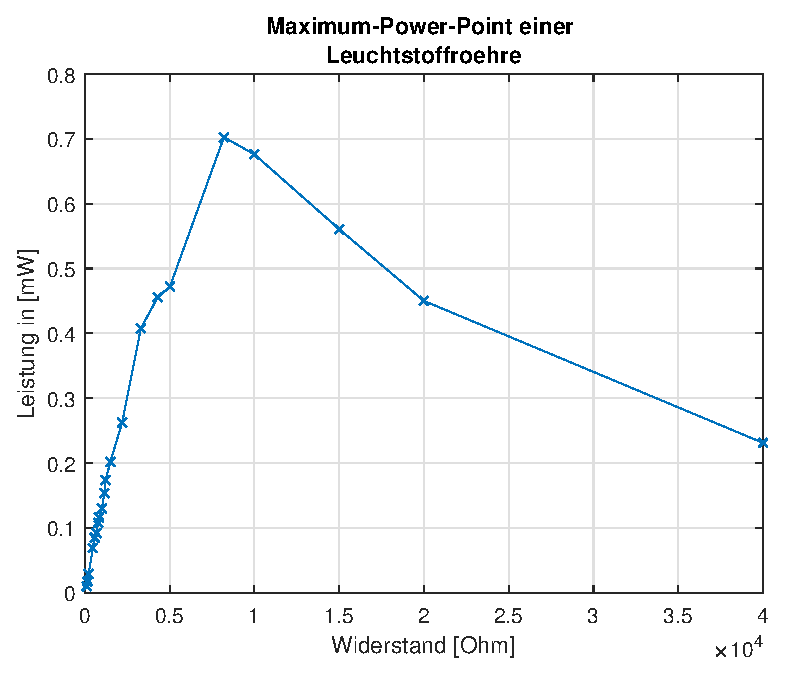
\includegraphics[width=11cm]{pictures/MPP/Leuchtstoffroehre-MPP.eps}
\caption{MPP einer Leuchtstoffroehre bei \SI{8200}{\ohm} und \SI{0.7024}{\milli \watt}}
\label{fig:I_U_Leuchtstoffroehre}
\end{figure}

\clearpage
\begin{figure}[htb]
\centering
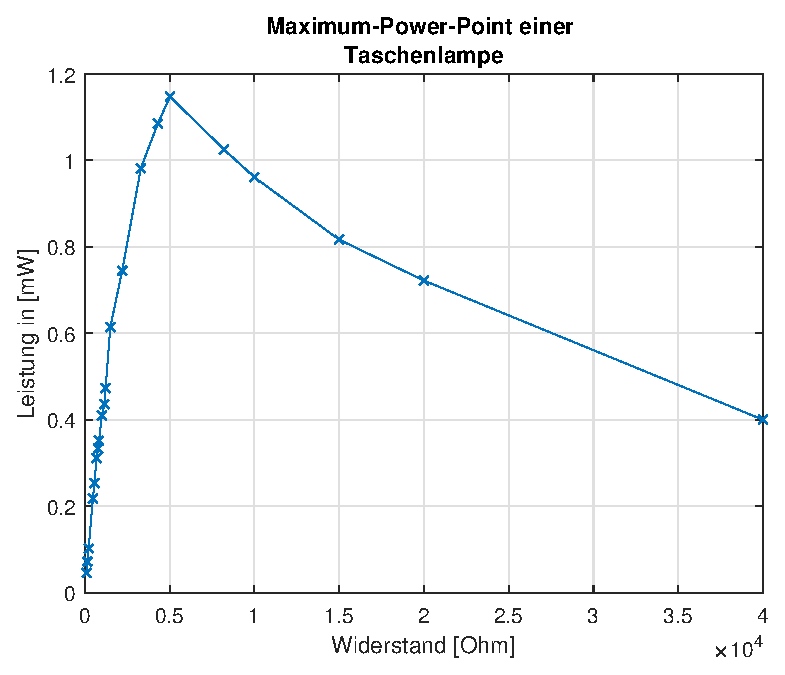
\includegraphics[width=11cm]{pictures/MPP/Taschenlampe-MPP.eps}
\caption{MPP einer Taschenlampe bei \SI{5020}{\ohm} und \SI{1.147}{\milli \watt}}
\label{fig:I_U_Taschenlampe}
\end{figure}

\begin{figure}[htb]
\centering
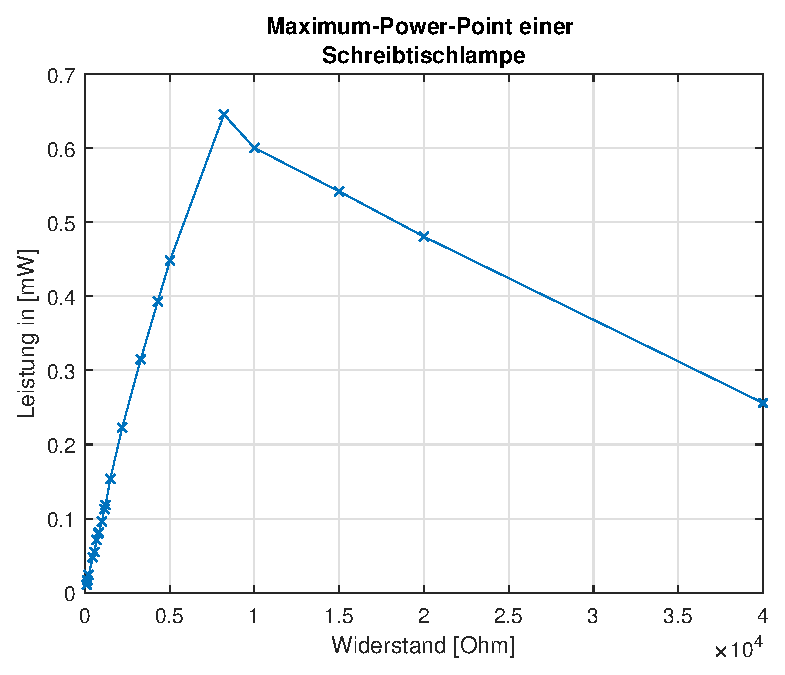
\includegraphics[width=11cm]{pictures/MPP/Schreibtischlampe-MPP.eps}
\caption{MPP einer Schreibtischlampe bei \SI{8200}{\ohm} und \SI{0.6451}{\milli \watt}}
\label{fig:I_U_Schreibtischlampe}
\end{figure}

\clearpage
\begin{figure}[htb]
\centering
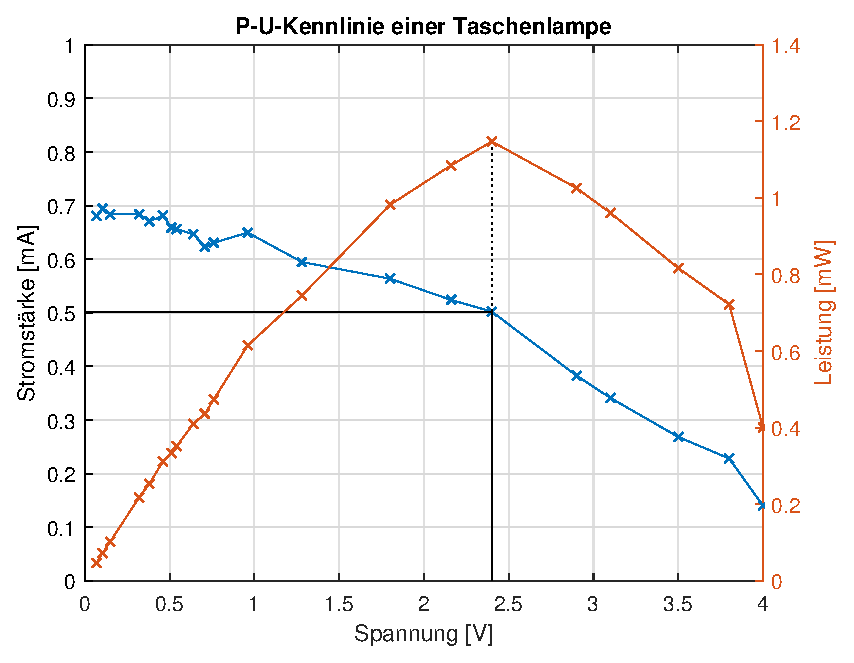
\includegraphics[width=11cm]{pictures/MPP/P-U-Kennlinie-Taschenlampe-MPP.eps}
\caption{P-U-Kennlinie einer Taschenlampe}
\label{fig:P-U-Kennlinie-Taschenlampe}
\end{figure}

\noindent{\Large Diskussion:\par}

Die Kurven der Leistung und der daraus ablesbare MPP entsprechen unseren Erwartungen und Messkurven aus dem a) Teil der Aufgabe.
Im P-U-Diagramm kann man deutlich sehen, dass der MPP an der Stelle der maximalen Leistung liegt.

\subsubsection{MPP-Anpassung}

Ein Solarwechselrichter ermittelt dynamisch den MPP einer Solarzelle und passt den Lastwiderstand so an, sodass die U-I-Kennlinie genau den MPP trifft und die Leistungsabgabe somit maximal ist.
Nach Möglichkeit sollte der MPP so oft wie möglich ermittelt werden, da die Bestrahlung der Solarzelle in der Praxis oft schwankt (Witterungsbedingungen, Verschattung...). \cite{Fachkundebuch}

%Aufgabe 3
\clearpage
\subsection{Langzeitmessung}

Für die ganze Aufgabe 3 wurde der folgende Aufbau verwendet:

\begin{figure}[htb]
\centering
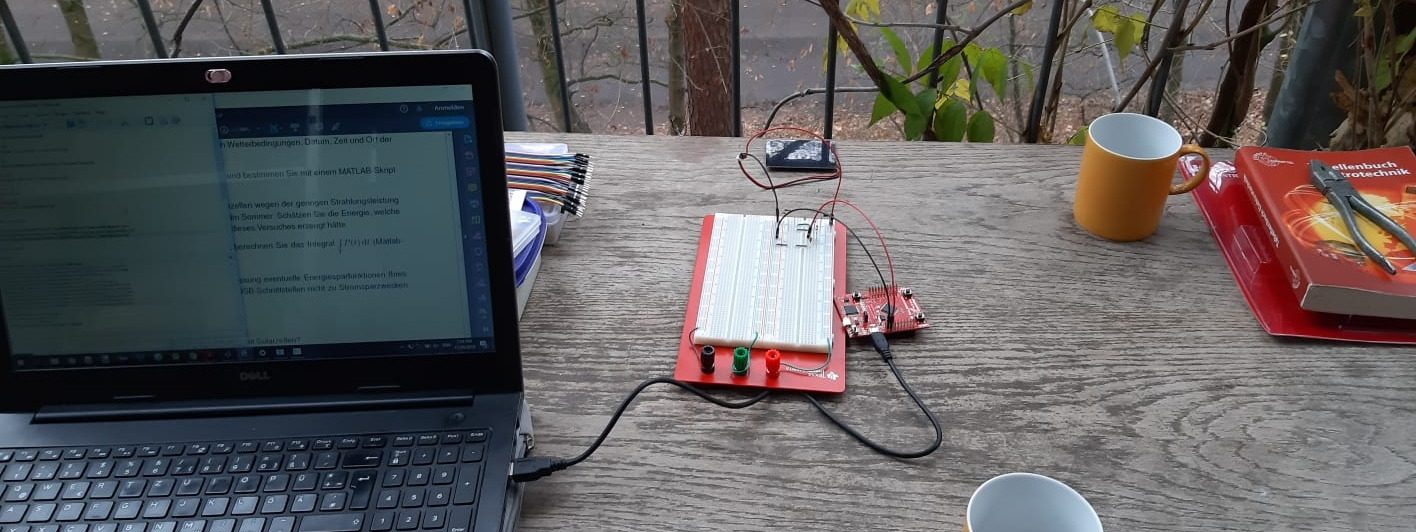
\includegraphics[width=16cm]{pictures/Dokumentation/Schaltung-2.jpeg}
\caption{Aufbau der Schaltung für die Aufgabe 3}
\label{fig:Schaltung3}
\end{figure}

Matlab-Skript zum Einlesen gemessener Werte:
\lstinputlisting[caption = Funktion \textit{importMessung.m}., label = importMessung.m]{matlab/importMessung.m}

\clearpage
\subsubsection{Spannungsverlauf \& Leistung}

\noindent{\Large Materialien:\par}

Messung durchgeführt am Donnerstag den 29. November 2018 von 13:20 Uhr bis 15:20 Uhr.
Wir rechnen mit einer Abnahme der Spannung, da die Messung nach 12:00 Uhr angefangen wurde und die Wintertage eine rapide Abnahme der Helligkeit aufweisen.

Wir erwarten deshalb, dass unsere U-t-Kennlinie über die Zeit abnimmt.
Die P-t-Kennlinie sollte einen ähnlichen Kurvenverlauf wie die U-t-Kennlinie darstellen, da $\frac{(U_{ges})^2}{\SI{1000}{\ohm}}$ gilt.

Matlab-Skript zur Ausgabe der Diagramme und der Energie:
\lstinputlisting[caption = Funktion \textit{LangzeitMessung.m}., label = LangzeitMessung.m]{matlab/LangzeitMessung.m}

\noindent{\Large Durchführung:\par}

\begin{table}[htb]
\centering
\caption{Bedingungen der Langzeitmessung}
\label{Langzeitmessung}
\begin{tabular}{c|cc}
\toprule
Uhrzeit & Wetterlage & Anmerkungen\\
\midrule
13:20 &  Teilweise verdeckter Himmel & Beginn der Messung\\
13:35 &  Himmel verdunkelt sich & Es tröpfelt\\
13:55 &  Himmel verdunkelt sich weiterhin & Regen aufgehört\\
14:15 &  Himmel lichtet sich etwas & \\
14:45 &  Sonne verschwindet wieder etwas hinter den Wolken & \\
15:20 &  Sonne kaum noch sichtbar & Ende der Messung\\
\bottomrule
\end{tabular}
\end{table}

Wetterbedingungen:

\begin{figure}[htb]
\centering
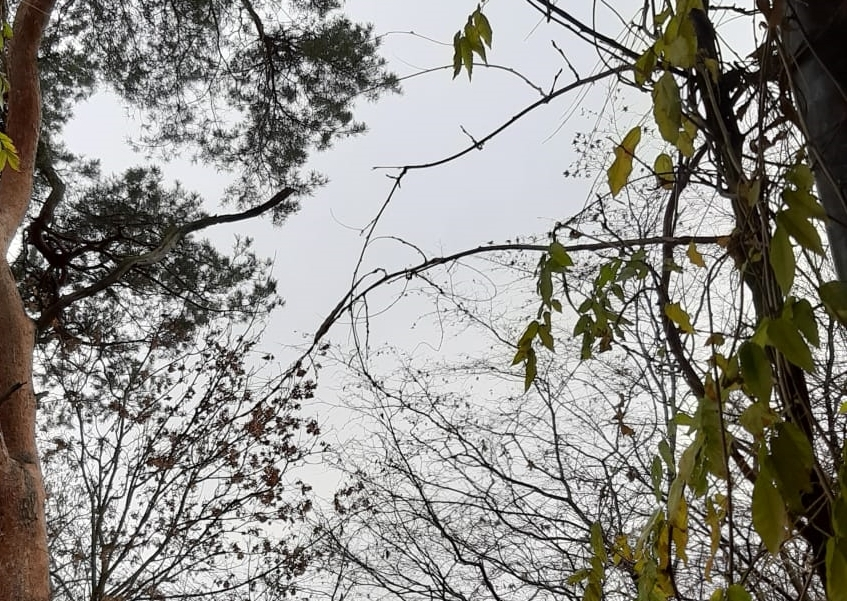
\includegraphics[width=16cm]{pictures/Dokumentation/Wetter.jpeg}
\caption{Wetterbedingungen bei der Langzeitmessung}
\label{fig:Wetter}
\end{figure}

\clearpage
\begin{figure}[htb]
\centering
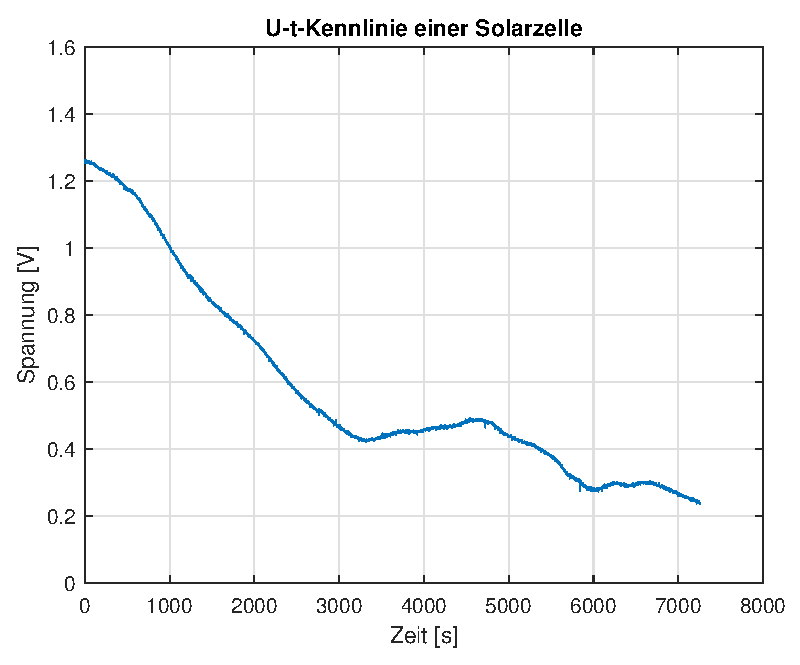
\includegraphics[width=12cm]{pictures/U-t/U-t-Kennlinie.eps}
\caption{U-t-Kennlinie der Langzeitmessung}
\label{fig:U-t-Kennlinie Langzeitmessung}
\end{figure}

\begin{figure}[htb]
\centering
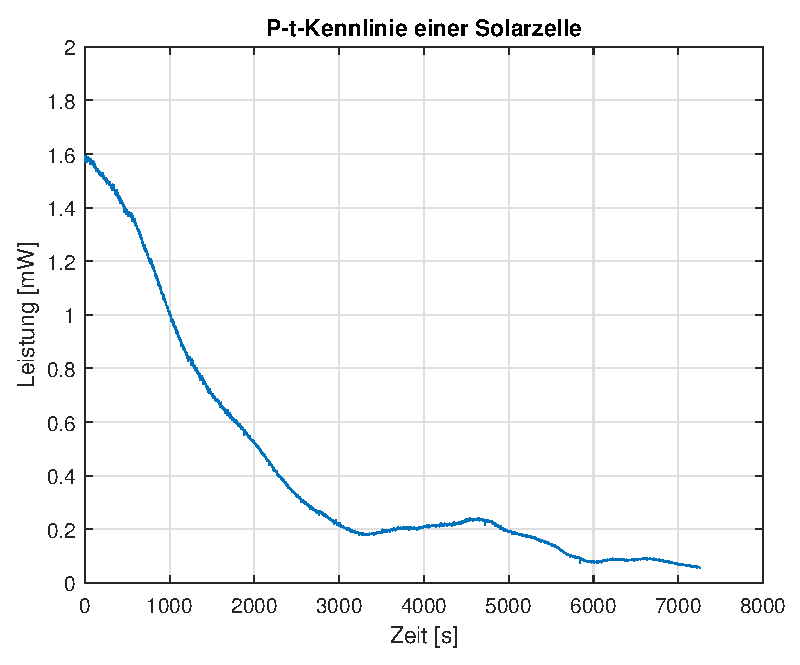
\includegraphics[width=12cm]{pictures/U-t/P-t-Kennlinie.eps}
\caption{P-t-Kennlinie der Langzeitmessung}
\label{fig:P-t-Kennlinie Langzeitmessung}
\end{figure}

\clearpage
Die Berechnung der Energie erfolgt mit der folgenden Formel: $\int\limits _T P(t)dt$ und ergibt ein Ergebnis von \SI{3074.3092}{\milli\watt\second}

\noindent{\Large Diskussion:\par}

Die Werte der U-t-Kennlinie verhalten sich wie erwartet: sie nehmen über die Zeit ab.
Die kleinen Sattelpunkte sind dabei die durch die Dynamik der Wolken zu erklären, welche die Sonne mehr oder weniger verdecken.
Auch die P-t-Kennlinie ähnelt wie erwartet in ihrer Form der U-t-Kennlinie.

Nun fällt auf, dass im Winter die Energiegewinnung durch eine Solarzelle weitaus geringer sein muss, als im Sommer.
Aus unseren vorherigen Messungen geht hervor, dass eine höhere Strahlungsintensität deutlich mehr Energie erzeugt.
Wir schätzen daher, dass die Energiegewinnung an einem sonnigen Sommertag bis zu 10-mal größer sein kann als an unserem bewölkten Wintertag.

\subsubsection{(Energiegewinnung)}

Wenn man die Ergebnise aus allen vorherigen Aufgaben betrachtet, so spielen viele Faktoren eine Rolle bei der Energiegewinnung durch eine Solarzelle. So hängt die gewonnene Leistung von dem erzeugten Strom und der daraus resultierenden Spannung ab, welcher wiederrum hauptsächlich durch die Strahlungsintensität bestimmt wird. Dabei haben Witterungsbedingungen wie die Lichtmenge oder der Einfallswinkel des Lichtes einen großen Einfluss.
Die Energie hängt aber auch vom Lastwiderstand der Solarzelle ab. Deshalb spielt der Einsatz bzw. die Effizienz eines Solarwechselrichters auch eine große Rolle, da er die Leistung der Solarzelle optimieren kann.

%Aufgabe 4
\clearpage
\subsection{Energiespeicherung \& Verhalten von Solarzellen}

\subsubsection{Theoretische Betrachtung}

Die gespeicherte Ladung eines Kondensators wird bei Belastung abgegeben, er entlädt sich also. Daraus resultiert eine Spannung, welche einen Stromfluss indiziert. Der Stromfluss nimmt dabei in seiner Intensität exponentiell ab. Durch den Ladungsausgleich (in Form eines Stromflusses) folgt ein Rückgang der anliegenden Spannung, welcher einen Rückgang des Stromflusses zur Folge hat. Bei einem polaren Kondensator ist der Stromfluss der Spannung entgegengerichtet.
Nach $5\tau$ ist der Kondensator annähernd komplett entladen. \cite{Fachkundebuch}

Folgende Formel kann in der Theorie zur Berechnung der Zeitkonstante verwendet werden:
\[
\tau = C * R = \SI{220}{\milli\farad} * \SI{500}{\ohm} = \SI{0.22}{\farad} * \SI{500}{\ohm} = \SI{110}{\second}
\]
Nach $5 * \SI{110}{\second} = \SI{550}{\second}$ ist der Kondensator der Theorie nach vollständig geladen bzw. entladen.
Praktisch gesehen ist der Kondensator jedoch schon vor $5\tau$ vollständig entladen wie man der praktischen Kurve ablesen kann. \cite{Fachkundebuch}

Folgendes Skript berechnet die theoretische Entladung des Kondensators:
\lstinputlisting[caption = Funktion \textit{KondensatorTheorie.m}., label = KondensatorTheorie.m]{matlab/KondensatorTheorie.m}

\begin{figure}[htb]
\centering
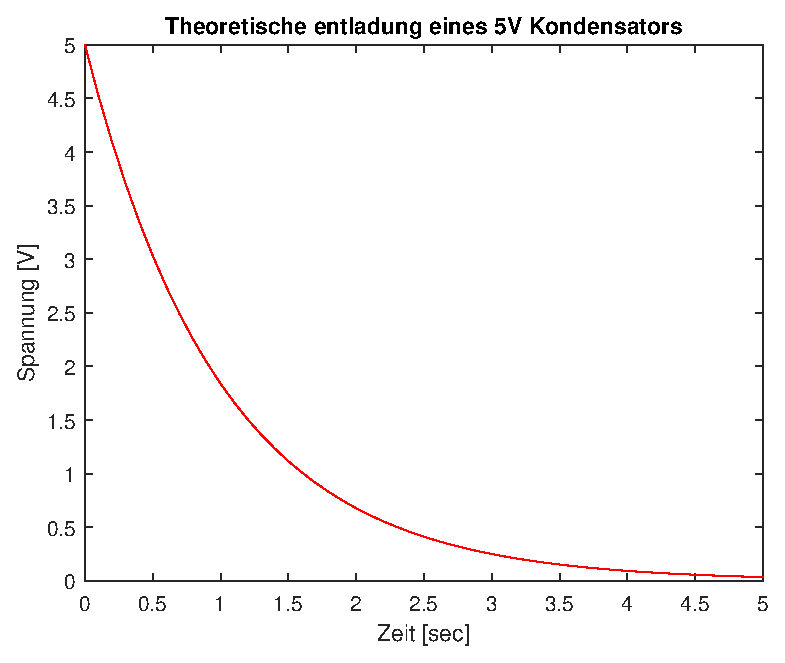
\includegraphics[width=14cm]{pictures/Kondensator/5-V-Theorie.eps}
\caption{Theoretische Entladung eines 5V-Kondensators}
\label{fig:entladung-theorie}
\end{figure}

\clearpage
\subsubsection{Messung \& Modellbildung}

\noindent{\Large Materialien:\par}

Wir erwarten, dass unsere Messkurve zur Entladung des Kondensators der theoretischen Kurve ähnelt, also exponentiell verläuft. Wir erwarten außerdem, dass unsere Ladungskurve der Ladungskurve an der x-Achse gespiegelt entspricht.

Zum Einlesen der Messwerte wurde das Matlab-Skript aus Aufgabe 3 verwendet: Quellcode \ref{importMessung.m}

\noindent{\Large Durchführung:\par}

Folgendes Skript wurde geschrieben, um ein U-t-Diagramm des Aufladen und des Entladend des Kondensators zu erstellen:
\lstinputlisting[caption = Funktion \textit{AufladenEntladen.m}., label = AufladenEntladen.m]{matlab/AufladenEntladen.m}

\begin{figure}[htb]
\centering
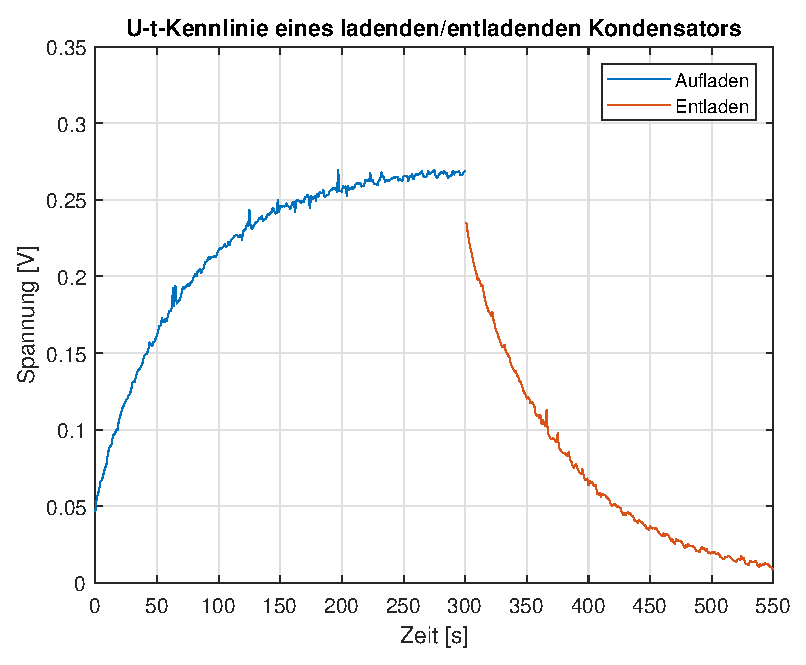
\includegraphics[width=12cm]{pictures/Kondensator/Aufladen-Entladen.eps}
\caption{Praktische Aufladung und Entladung eines Kondensators}
\label{fig:entladung-praxis}
\end{figure}

\clearpage
\noindent{\Large Diskussion:\par}

Unsere gemessene Entladungskurve entspricht bzw. ähnelt der theoretisch berechneten Entladungskurve. Auch unsere Ladungskurve entspricht der an der x-Achse gespiegelten Entladungskurve. Somit liegen unsere gemessenen Werte in unserem Erwartungsbereich
\\
\\
Die Ladungskurven hängen von der Bauweise des Kondensators ab. 
Bei steigender Ladung wächst der Innenwiderstand des Kondensators, somit reduziert sich der Stromfluss je weiter die Ladung voranschreitet. Ab einem gewissen Punkt ist der Kondensator voll geladen und kann keine weitere Ladung mehr aufnehmen. Daraus ergibt sich eine Kurve des begrenzten Wachstums.
Bei der Entladung gibt der Kondensator seine Ladung ab. Dabei ähnelt er einer endlichen Spannungsquelle. Je mehr Ladung er abgibt, desto geringer wird die Spannung welche er indiziert. Daraus ergibt sich die Kurve des fallenden Wachstums.
Auch bei den I-U-Kennlinien kann man dieses Phänomen beobachten. Mit einem steigenden Lastwiderstand nimmt die Stromstärke bei steigender Spannung ab. Betrachtet man den Kondensator als Widerstand, welcher durch seine Ladung bestimmt wird, so stellt ein voll geladener Kondensator einen unendlich hohen Widerstand dar, wobei man nun an den I-U-Kennlinien eine quasi nicht vorhandene Gesamtstromstärke durch den Kondensator ablesen kann.
\\
\\
Die Solarzelle stellt eine Stromquelle dar. Dies erkennt man zum Beispiel an den I-U-Kennlinien, durch die bis zu einem gewissen Widerstand ein konstanter Strom bei unterschiedlicher Spannung geliefert wird.
\\
\\
Gewonnene Ladungsenergie: $\int\limits _T (U(t) * (C * \frac{\Delta U(t)}{\Delta t}))dt = $ \SI{33.3798}{\milli\watt\second}\\
Verbrauchte Entladungsenergie: $\int\limits _T (U(t) * (C * \frac{\Delta U(t)}{\Delta t}))dt = $ \SI{-27.7073}{\milli\watt\second}\\
Wirkungsgrad: $\frac{\SI{27.7073}{\milli\watt\second}}{\SI{33.3798}{\milli\watt\second}} * 100 ~= 83.01\%$\\
\\
Der errechnete Wirkungsgrad des Kondensators ist schlecht, da ca. 15\% der Energie verloren geht. Dies ist besonders bei Solarzellen tragisch, welche schon einen sehr geringen Wirkungsgrad haben. Dies veranschaulicht sehr gut, weshalb Energiespeicherung mit Batterien bzw. Akkus realisiert wird und nicht mit Kondensatoren.

\clearpage
\subsubsection{Gesamtenergie \& Wirkungsgrad}

\noindent{\Large Materialien:\par}

Wir erwarten, dass beim An- bzw. Abschalten der Solarzelle ohne Kondensator steile Flanken bei der Messung abzulesen sind, da die erzeugte Spannung entweder vorhanden oder nicht vorhanden ist und demnach nicht gespeichert wird.
Bei dem Messaufbau mit Kondensator erwarten wir ein langsames Abfallen der Spannung nach Verschattung der Solarzelle nach der Charakteristik der Entladungskurve des Kondensators (siehe vorherige Aufgabe). Beim Beleuchten der Solarzelle lädt sich der Kondensator erstmal auf, wir erwarten deshalb eine charakteristische Ladekurve des Kondensators zu Beginn der Messung und eine Sägezahnähnlichen Verlauf während der An- und Abschaltphase.

Folgendes Skript wurde geschrieben, um die U-t-Diagramme der Solarzelle mit und ohne Kondensator zu generieren:
\lstinputlisting[caption = Funktion \textit{VergleichEnergiespeicher.m}., label = VergleichEnergiespeicher.m]{matlab/VergleichEnergiespeicher.m}

\clearpage
\noindent{\Large Durchführung:\par}

\begin{figure}[htb]
\centering
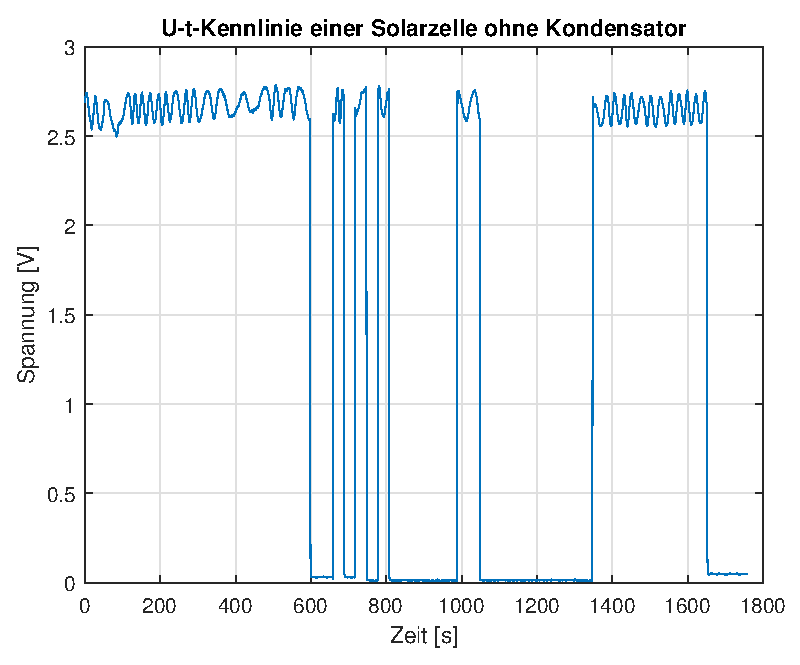
\includegraphics[width=11cm]{pictures/Vergleich/ohne-Kondensator.eps}
\caption{U-t-Diagramm einer Solarzelle ohne Kondensator}
\label{fig:ohne-Kondensator}
\end{figure}

\begin{figure}[htb]
\centering
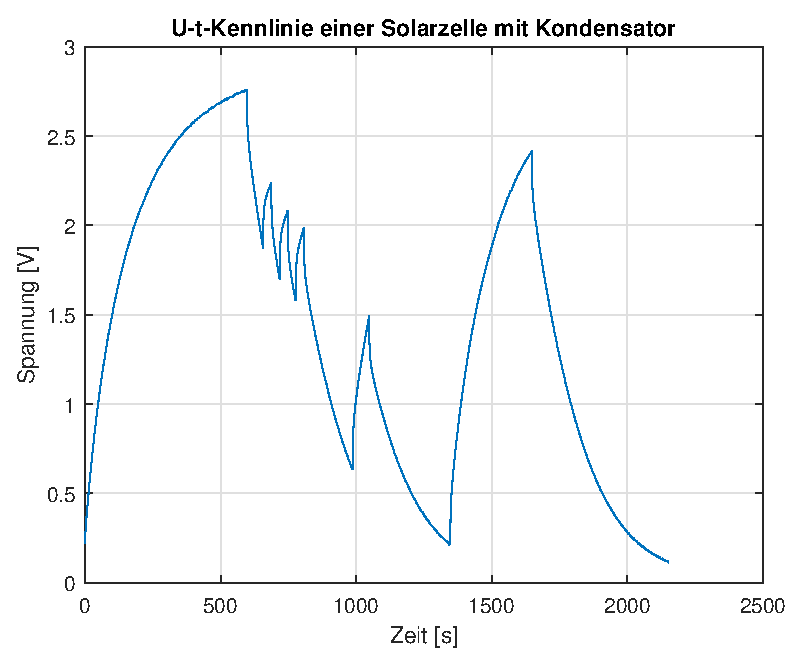
\includegraphics[width=11cm]{pictures/Vergleich/mit-Kondensator.eps}
\caption{U-t-Diagramm einer Solarzelle mit Kondensator}
\label{fig:mit-Kondensator}
\end{figure}

\clearpage
\section{Zusammenfassung}

Bei der Messung ohne Kondensator sind die Abfälle der Spannung wie erwartet steil bzw. direkt. 
Die Messkurven stimmen mit unseren Erwartungen überein. Zu Beginn der Messung mit Kondensator ist eine typische Ladekurve des Kondensators ablesbar, zum Ende der Messung eine typische Entladungskurve. Im Bereich der 30-Sekunden-Beleuchtung sinkt die Spannung, welche der Kondensator bei keiner Beleuchtung abgibt schneller, als die Spannung welche der Kondensator bei Beleuchtung aufnimmt.
\\
\\
Speicherkondensatoren eignen sich für manche Anwendungen, in denen zum Beispiel kurzzeitige Spannungseinbrüche überbrückt bzw. ausgeglichen werden sollen.
Zur reinen Energiespeicherung über einen längeren Zeitraum bei großen Ladungsmengen eigenen sie sich jedoch nicht. Hierfür ist es sinnvoller auf Batterien oder Akkus zurückzugreifen. Dies kann dadurch erklärt werden, dass ein Kondensator seine Ladung schnell abgibt und keine Spannung über einen längeren Zeitraum aufrecht halten kann (siehe die Entladungskurve des Kondensators Abbildung [\ref{fig:entladung-praxis}]). 
Außerdem können Kondensatoren keine konstante Spannung und keinen konstanten Strom liefern, was sie für langfristige Energiequellen ungeeignet macht.
Für große Anwendungen bzw. bei Verwendung großer Energiemengen (zum Beispiel Fahrzeuge, Maschinen, etc.) eignen sich Kondensatoren kaum, da sie die nötige Energie nicht liefern können. Um diesen Zwecken gerecht zu werden bräuchte man Unmengen an Kondensatoren oder unendlich große Kondensatoren. Deshalb bieten sich Akkus und Batterien in jeder Hinsicht besser zur Energiespeicherung an als Kondensatoren.
\\
\\
Das hauptsächliche Ziel der Energiespeicherung ist die möglichst verlustfreie Aufnahme und Abgabe von Energie zu unterschiedlichen Zeitpunkten. Dabei soll speziell die Energieabgabe linear erfolgen, um eine optimale Strom- bzw. Spannungsquelle zu imitieren. Dadurch kann die abgegebene Energie auch optimal genutzt werden.
Als Beispiel kann eine Solarzelle betrachtet werden. Sie generiert bei Sonnenlicht Strom, wobei bei Sonnenlicht weniger Energie (durch Licht, Wärme, etc.) gebraucht wird. Bei keinem Sonnenlicht generiert die Solarzelle keinen Strom, dieser wird jedoch benötigt. Aufgrund dessen ist es wichtig, Energie bei Energieüberschüssen abzugreifen und Energie im Falle von Energiebedarf abzugeben.
\\
\\
Hierbei gibt es drei Hauptpunkte, welche verbessert werden können: der Wirkungsgrad des Speichers, die gleichmäßige Entladung bzw. Aufladung und die allgemeine Kapazität des Speichers.
Eine höhere Kapazität kann durch eine größere Fläche eines Speicherkondensators oder durch größere Zellen einer Batterie oder das kombinieren von Speichern erreicht werden.
Der Wirkungsgrad kann durch verschiedene Baustoffe oder Konstruktionsweisen der Batterien oder der Kondensatoren optimiert werden.
Eine besonders gleichmäßige Entladung kann durch einen optimal gewählten Lastwiderstand erreicht werden.